% !TEX TS-program = pdflatex
% \documentclass[draftcls, onecolumn, journal]{IEEEtran}
% \documentclass[journal]{IEEEtran}
\documentclass[a4paper,11pt]{article}
%\usepackage{fullpage}

%\renewcommand{\baselinestretch}{1.9}
\usepackage{graphicx}
%\usepackage{cite}
\usepackage[style=ieee, nohashothers=true, nosortothers=true, uniquelist=true, natbib=true, backend=biber, sorting=none]{biblatex}
\DefineBibliographyStrings{english}{andothers={}}

\addbibresource{project.bib}
\DeclareFieldFormat[article]{volume}{Vol. #1}
\DeclareFieldFormat[article]{number}{No. #1}
\DeclareFieldFormat[article]{pages}{p. #1}
\DeclareFieldFormat[inproceedings]{pages}{p. #1}

%\documentclass[journal]{IEEEtran}
\usepackage[a4paper, total={6in, 8.5in}, top=1in, bottom=1in, left=1in, right=1in]{geometry}
\usepackage{mathtools}
\usepackage{amssymb}
\usepackage{amsmath}
\usepackage{pythonhighlight}
\usepackage[utf8]{inputenc}
\usepackage{fancyhdr}
\usepackage{pythonhighlight}
\usepackage{changepage}
\usepackage{slashbox}
\usepackage{floatrow}
\usepackage{listings}
\usepackage[hidelinks]{hyperref}
\usepackage[T1]{fontenc}
\usepackage[utf8]{inputenc}
\usepackage[english]{babel}
\usepackage{csquotes}
\usepackage{booktabs}
\usepackage{multicol}
\usepackage{titlesec}
\usepackage{fontawesome5}
\usepackage{makecell}
\usepackage{footnote}

\setcounter{secnumdepth}{4}
\setcounter{tocdepth}{4}


\titleformat{\paragraph}
{\normalfont\normalsize\bfseries}{\theparagraph}{1em}{}
\titlespacing*{\paragraph}
{0pt}{3.25ex plus 1ex minus .2ex}{1.5ex plus .2ex}

\usepackage{caption}
\usepackage{subcaption}
\usepackage{color} %red, green, blue, yellow, cyan, magenta, black, white
\definecolor{mygreen}{RGB}{28,172,0} % color values Red, Green, Blue
\definecolor{mylilas}{RGB}{170,55,241}


\floatsetup[table]{capposition=top}

\sloppy
\definecolor{lightgray}{gray}{0.5}
\setlength{\parindent}{0pt}
\setlength{\headheight}{14pt}

\renewcommand{\headrulewidth}{.4mm} % header line width
\newcommand{\norm}[1]{\left\lVert#1\right\rVert}
\renewcommand\footnoterule{\kern-3pt \hrule width 3in \noindent \kern 2.6pt}


\pagestyle{fancy}
\fancyhf{}
\fancyhfoffset[L]{-1cm} % left extra length
\fancyhfoffset[R]{-1cm} % right extra length
\rhead{\bfseries Kutay U\u{g}urlu 2232841}
\lhead{Deep MLP for Dimensional SER}
\rfoot{}

\DeclarePairedDelimiter\ceil{\lceil}{\rceil}
\DeclarePairedDelimiter\floor{\lfloor}{\rfloor}

\author{Kutay U\u{g}urlu 2232841}

\begin{document}

    
\lstset{language=Matlab,%
    %basicstyle=\color{red},
    breaklines=true,%
    morekeywords={matlab2tikz},
    keywordstyle=\color{blue},%
    morekeywords=[2]{1}, keywordstyle=[2]{\color{black}},
    identifierstyle=\color{black},%
    stringstyle=\color{mylilas},
    commentstyle=\color{mygreen},%
    showstringspaces=false,%without this there will be a symbol in the places where there is a space
    numbers=left,%
    numberstyle={\tiny \color{black}},% size of the numbers
    numbersep=9pt, % this defines how far the numbers are from the text
    emph=[1]{for,end,break},emphstyle=[1]\color{red}, %some words to emphasise
    %emph=[2]{word1,word2}, emphstyle=[2]{style},    
}

\fancyfoot[C]{\thepage}

\title{\LARGE \LARGE EE583 Pattern Recognition Project \\ 
Analaysis of \textit{Deep Multilayer Perceptrons for Dimensional Speech Emotion Recognition}}

\maketitle{\LARGE}
\pagebreak
\tableofcontents
\listoffigures
\listoftables
\pagebreak

\section{Introduction}

Speech emotion recognition is the task of extracting the emotion category from either text or audio data. It has already some applications in security, medicine, entertainment and education \cite{cen2016real}. 

This project report investigates the idea that Atmaja \textit{et al.}stated in \textit{Deep Multilayer Perceptrons for Dimensional Speech Emotion Recognition}~\cite{atmaja2020deep}. The authors of the study discusses the need of utilizing modern computation units, such as Long Short Term Memory(LSTMs) and Convolutional Neural Networks(CNNs), in the neural networks for the task of dimensional speech emotion recognition. The authors state in the Conclusion section of their paper that the future research should be directed to evaluate the cross corpus evaluations. In this project, the proposed method is evaluated on both other corpora and between-corpora. 
\\
\\
The organization of the report is as follows:
\begin{itemize}
    \item The problem and the proposed solutions to it are briefly introduced in this section.
    \item The theory of dimensional and categorical emotions are mentioned in Section \ref{sec:theory}.
    \item The methods, datasets and neural network architectures used in the implementation of the original paper along with modifications introduced in the speech emotion recognition tasks can be seen in Section \ref{sec:implementation}.
    \item Section \ref{sec:results} is left for the presentation of the results from conducted experiments along with the reproduced results, and a discussion on them with a focus on comparison of the models.   
\end{itemize}



\section{Theory} \label{sec:theory}

\begin{figure}[h]
    \centering
    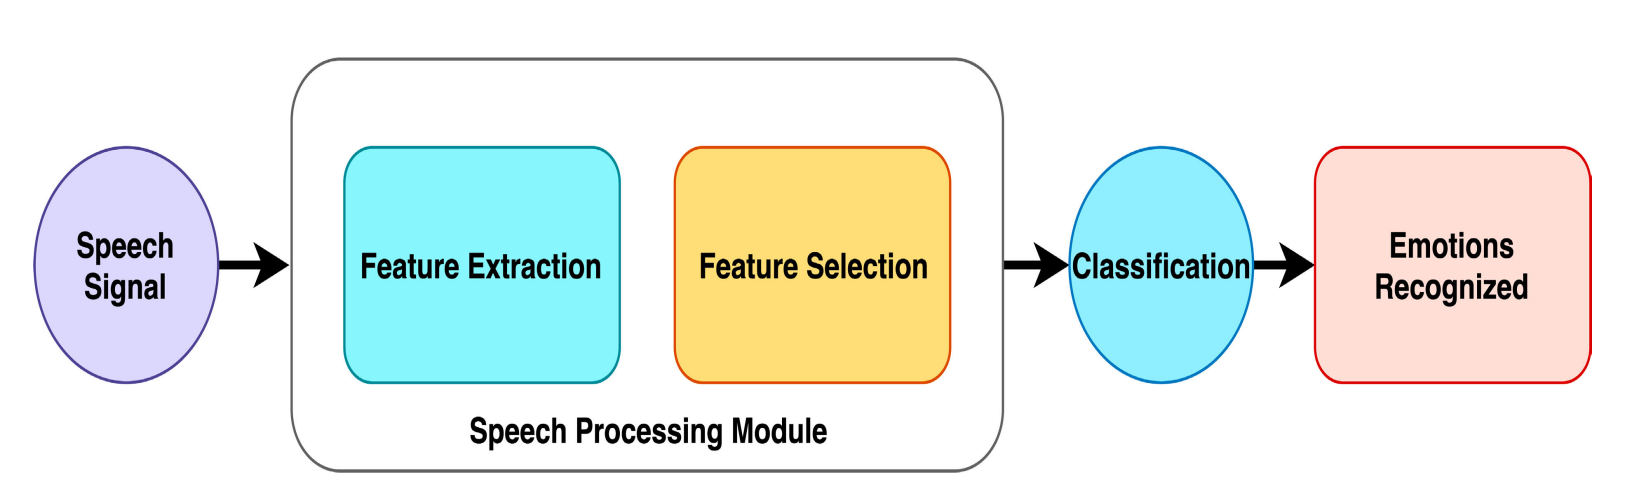
\includegraphics[width=1\textwidth]{chart.png}
    \caption{Traditional Speech Emotion Recognition Scheme \cite{ser_deep_dl}}\label{fig:traditional}
\end{figure}

The traditional algorithm for speech emotion recognition is demonstrated in Figure \ref{fig:traditional}. Unlike these scheme, authors used to convert this categorical classification problem to a regression problem by using the dimensional emotion concept. In other words, they first predicted the magnitude of an utterance in each dimension. The remaining classification task afterwards is just deciding on which category an utterance belongs to in the dimensional emotion feature space. 

\pagebreak

The idea that emotion categories can be classified based on some emotional dimensions dates back to 1979. Russel argued in \cite{russell1979affective} that categorical emotions, namely sadness, anger, joy, etc., can be classified by the values they represent in three dimensions: Valence, Arousal and Dominance.

\begin{figure}[h]
\centering
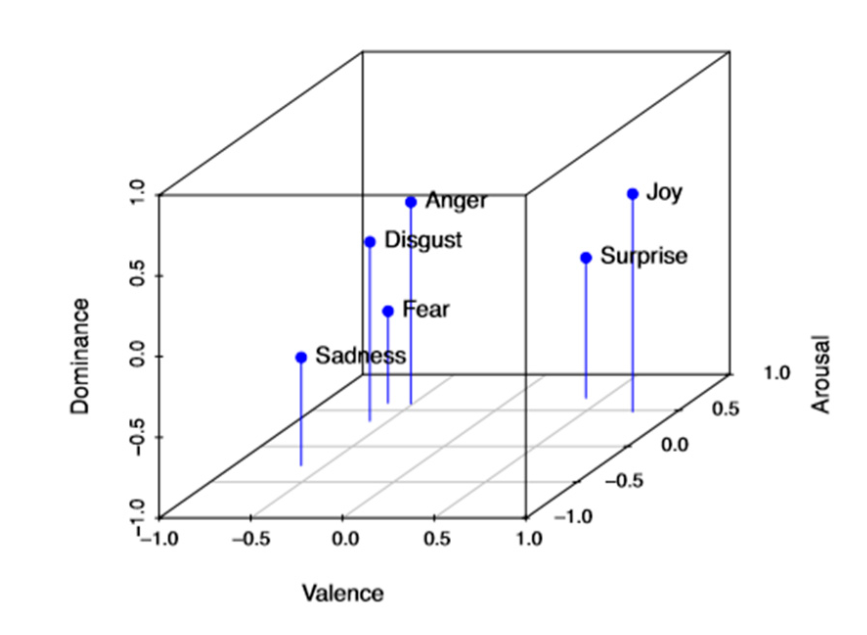
\includegraphics[width=0.8\textwidth]{dimensions_pic.png}
\caption{Categorical Emotions in VAD space \cite{bualan2020emotion}}\label{fig:dimensions}
\end{figure}

\begin{table}[h]
    \centering{
\begin{tabular}{cccc} \toprule \toprule
     & Valence & Arousal & Dominance \\ \midrule
    Anger  & -0.43 & 0.67 & 0.34  \\ \midrule
    Joy  & 0.76  & 0.48 & 0.35   \\ \midrule
    Surprise  & 0.4  & 0.67 & -0.13   \\ \midrule
    Disgust  & -0.6  & 0.35 & 0.11   \\ \midrule
    Fear  & -0.64   & 0.6 & -0.43    \\ \midrule
    Sadness  & -0.63  & 0.27 & -0.33   \\ \bottomrule \bottomrule
\end{tabular}
}
\caption{\label{tab:vadtable}VAD Dimensions of 6 basic emotions \cite{bualan2020emotion}.}
\end{table}

The categorical emotions of a given utterance can be decided based on its dimensional features' location in the Valence-Arousal-Dominance space. The authors of the study show that by using this idea, the Multilayer Perceptrons networks achieve more success, although being obsolete and computationally less costly, compared to more modern computational units such as LSTMs and CNNs, provided that the same number of architecture units are used and resultant number of parameters are not significantly different.

\pagebreak

\section{Implementation} \label{sec:implementation}

This section composes of two sections describing the implementation of the original authors and slight changes made.

\subsection{Original Paper}
\subsubsection{Data} 

\paragraph{Datasets}

There are mainly two datasets utilized in the paper. 
\begin{enumerate}
    \item \textbf{IEMOCAP(The Interactive emotional Dyadic Motion Capture database):} 12 hours of speech data consisting of 10039 utterances  is used \cite{busso2008iemocap}.
    \item \textbf{MSP-IMPROV:} 18 hours of speech data consisting of 8438 utterances is used \cite{busso2016msp}.
\end{enumerate}

\paragraph{Data Preprocessing} \label{subsec:datapreprocess}

The shared data in \cite{atmaja2020deep} are already preprocessed and the scripts and tools the authors utilized was not explicitly shared. However, the types of features Atmaja \textit{et al.} used is shared in the paper.  
The audio in the dataset are used to extract 47 features per utterance.
These features are obtained in a 2-level process. First, the Low Level Descriptors defined in \cite{eyben2010opensmile} are calculated by the \texttt{opensmile} software. These Low Level Descriptors are as follows: 
\begin{multicols}{2}
\begin{itemize}
    \item Intensity
    \item Alpha ratio
    \item Hammarberg index
    \item Spectral slope 0-500 Hz
    \item Spectral slope 500-1500 Hz
    \item Spectral flux
    \item 4 MFCCs
    \item $f_0$
    \item jitter
    \item shimmer
    \item Harmonics-to-Noise Ratio (HNR)
    \item Harmonic difference H1-H2
    \item Harmonic difference H1-A3
    \item F1
    \item F1 bandwidth
    \item F1 amplitude
    \item F2
    \item F2 amplitude
    \item F3 
    \item F3 amplitude
\end{itemize}
\end{multicols}

Then, 47 features, High Statistical Functions of these 23 features are calculated in two sets by utilizing the mean and standard deviation. In addition, authors defined an extra feature: Silence. The silence is defined as the ratio of the silent frames per utterance. 

\begin{align}
    S &= \frac{N_s}{N_t} & Threshold &= 0.3 \times X_{RMS}
\end{align}
where $N_s$ is the number of silent frames and $N_t$ is the number of total frames.
The frames are labelled as silent by being compared to a threshold whose factor 0.3 is determined empirically. 
\begin{align}
    X_{RMS} &= \sqrt{\frac{1}{n}\sum_{i=1}^n{x[i]}^2}
\end{align}

\paragraph{Scaling}
Both the data and the labels that were originally labelled in the range $[-5,5]$ are scaled to the range [-1,1] in ReLU activated CNNs and LSTM networks. 

\subsubsection{Models}

The benchmark models which authors use to compare the model performance are composed of CNN and LSTM units. The authors use the same number of units and layers in the model. In Figure \ref{fig:models}, it can be seen that the models have approximately the same number of trainable parameters. 
\\
\\
The multiplayer perceptron models are implemented with scikit-learn's MLP Regressor \cite{scikit-learn} and the remaining CNN and LSTM models are implemented with Tensorflow \cite{tensorflow2015-whitepaper}.

\begin{figure}[h]
\centering
\begin{subfigure}[b]{0.45\textwidth}
\centering
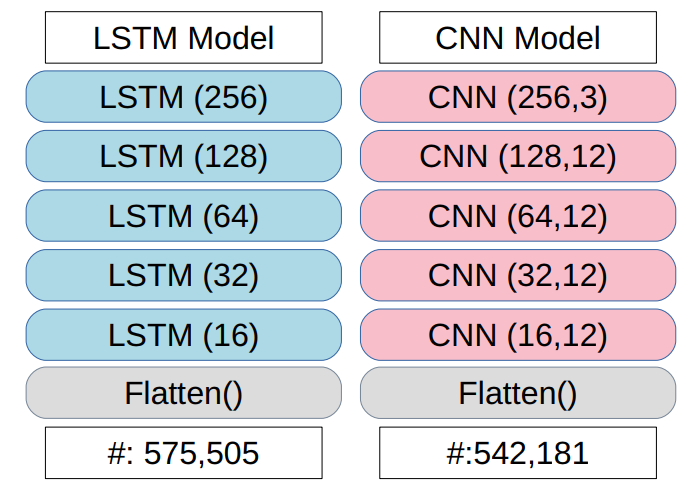
\includegraphics[width=0.8\textwidth, height=5cm]{modelsparams.png}
\caption{Benchmark model architectures}\label{subfig:subcnnlstm}
\end{subfigure}
\begin{subfigure}[b]{0.45\linewidth}
\centering
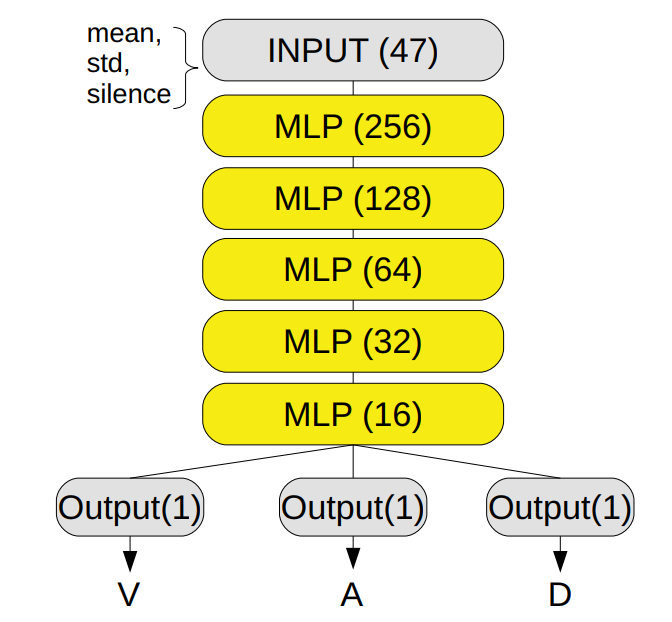
\includegraphics[width=0.8\textwidth]{modelparamsmlp.png}
\caption{Proposed Multilayer MLP architecture}\label{subfig:submlp}
\end{subfigure}
\caption{Model architectures utilized in \cite{atmaja2020deep}}
\label{fig:models}
\end{figure}

\paragraph{Loss Function: CCC Loss}

To optimize the network, Concordance Correlation Coefficient in Eqn. \ref{eq:CCC} is used. 
\begin{equation}
    CCC = \frac{2\rho{\sigma_x}{\sigma_y}}{{\sigma_x}^2 + {\sigma_y}^2 + (\mu_x - \mu_y)^2}
    \label{eq:CCC}
\end{equation}

Then, the loss can be found as $CCCL = 1 - CCC$.

The total loss with respect to this loss is defined to be the sum of loss of individual classes follows:
\begin{equation}
    CCCL_T = CCCL_V + CCCL_A + CCCL_D
    \label{eq:CCCLoss}
\end{equation}

However, the authors state that they could not find a way to implement this loss function to optimize MLP models. Hence, they used MSE Loss instead in the training process, and CCC Loss again in the evaluation. 

\begin{equation}
    MSE = \frac{1}{N}\sum_{i=1}^N (y_i -{\hat{y}}_i)^2
\end{equation}

\pagebreak

\subsection{Modifications}

The software provided in the \href{https://github.com/bagustris/deep_mlp_ser}{repository \faExternalLink*} \footnote{https://github.com/bagustris/deep\_mlp\_ser} is copied via \texttt{git clone} and some additional changes made on the repository. The modified version is shared \href{https://github.com/kutay-ugurlu/Analysis-of-Deep-MLP-SER}{here \faExternalLink*} \footnote{ https://github.com/kutay-ugurlu/Analysis-of-Deep-MLP-SER}.

\subsubsection{Data}\label{subsec:MELDdata}

\paragraph{Datasets}

The authors of the study made use of the most of the databases whose utterances are labelled by multiple annotators in the Valence-Arousal-Dominance dimension. 
Although there are many available datasets on Speech Emotion Recognition, only a few of them are labelled in the same manner. However, these datasets were not available for open access. The remaining available datasets are either labelled categorically, \textit{i.e.} sad, joy, anger etc. or labelled only in 2 dimension: Valence and Arousal. Since the latter option requires one to re-train the model, does not provide one with the chance of evaluating the pretrained model with the new test data and results in an unfair evaluation of the results since the dimension of the problem is changed, categorical dataset, MELD \cite{atmaja2020deep}, was used for the evaluation. The dataset consists of utterances in mp4 format from the TV series ''Friends'' and the categorical emotions regarding these utterances. The number of labeled utterances is 2610 for test and 5279 for training sets. However, the number of utterances labelled as ''neutral'' in the emotions, which corresponds to the origin of the Valence-Arousal-Dominance space, was exceedingly higher than the others, and it was causing problems in both class-imbalance sense and in the learning part of the regression networks, hence those samples were dropped from the dataset.

\begin{figure}[h]
\centering
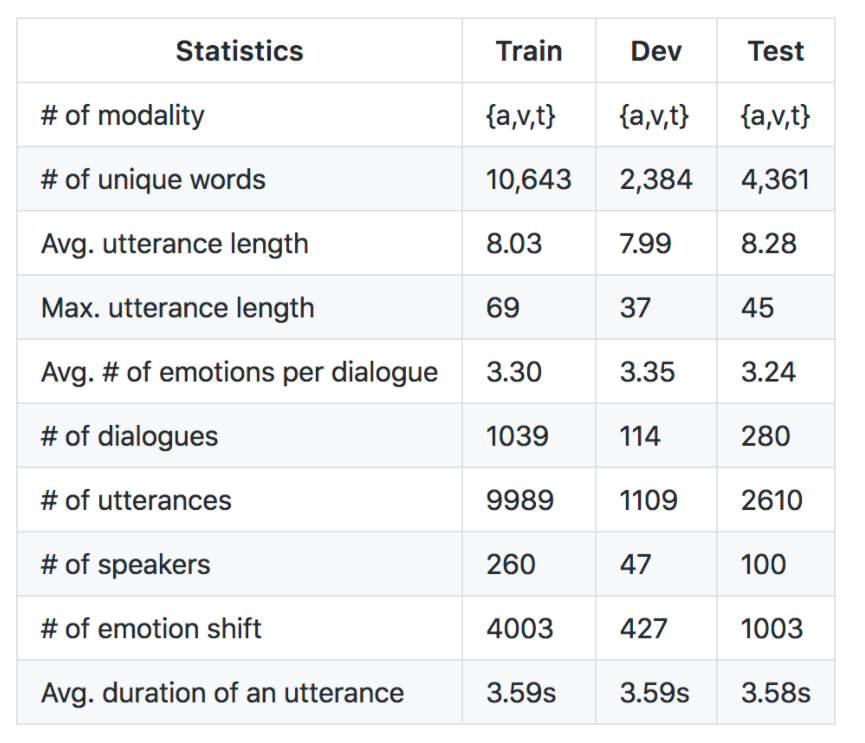
\includegraphics[width=0.8\textwidth]{MELDStats.png}
\caption{MELD Dataset statistics}\label{fig:meldstats}
\end{figure}

\paragraph{Data Preprocessing}

To augment the dimensional, \textit{i.e.} numerical, labels from the categorical labels. This is conducted by mapping the categorical labels to points in the Valence-Arousal-Dominance space via the mapping given in Table \ref{tab:vadtable} first, and perturbing the points with normally distributed noise with standard deviation 0.01, to reflect the effect of multiple annotators. To get the time series data in WAV format in the same sampling rate of 44.1 kHz from MP4 format, \texttt{FFMPEG} \cite{tomar2006converting} is utilized.   

The whole data formation process can be seen in Figure \ref{fig:dataformation}.

\begin{figure}[h]
\centering
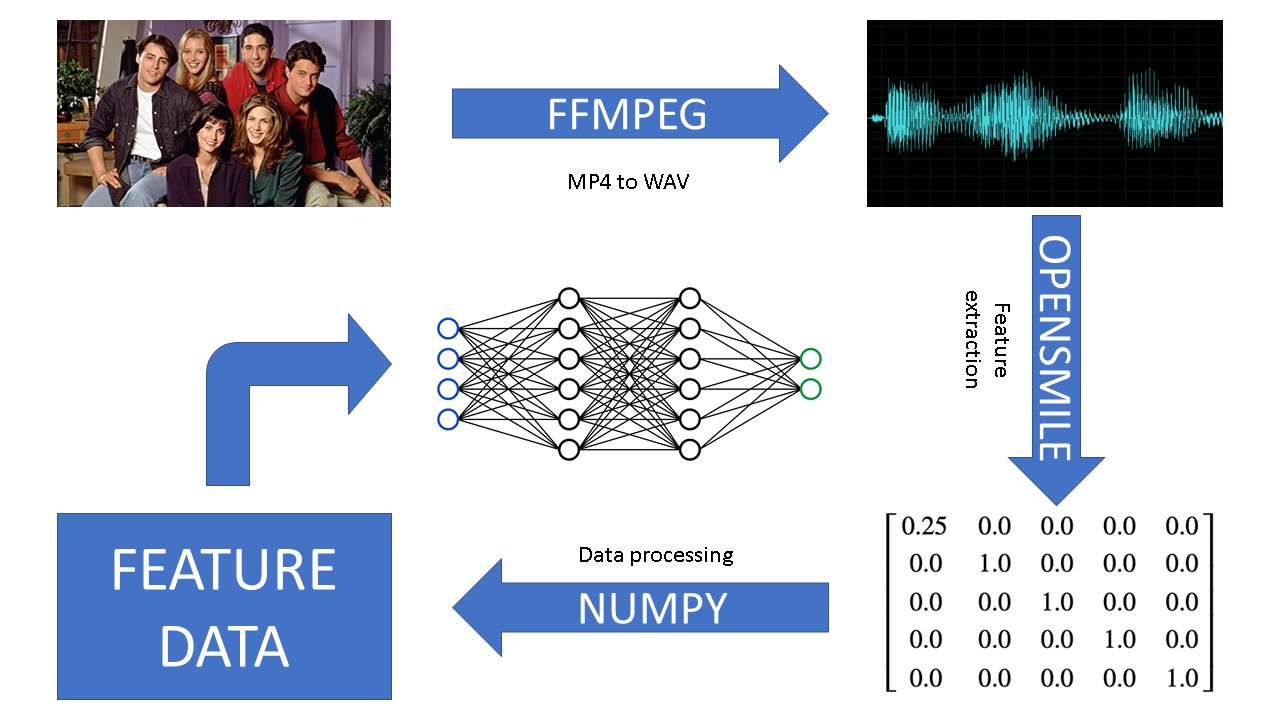
\includegraphics[width=0.6\textwidth]{Presentation.png}
\caption{The data formation steps used to augment data from MELD dataset}\label{fig:dataformation}
\end{figure}

The data processing steps shown above visually in Figure \ref{fig:dataformation} is explained in detail in section \ref{subsec:datapreprocess}.

\subsubsection{Models}

The pre-trained models are evaluated using the new test data. Furthermore, to make better conclusions on the models' capability to fit the data, the data is split to train, test and validation sets and the model is evaluated after being retrained. The architectures of the model were not changed. The only change made was the number of training and patience epoch for early stopping. The comparison was only made for speaker independent case due to the requirement of splitting the newly introduced test data in a speaker-wise manner and train the models using mixed datasets in the speaker dependent case and lack of available continuous data from the same speaker.

\pagebreak

\section{Results and Discussion} \label{sec:results}
\begin{table}[h]
    \centering
    \begin{tabular}{cccccc}
        \toprule
        {} &  \makecell{Original \\ Mean CCC} &  \makecell{Tested \\Valence CCC} &  \makecell{Tested \\Arousal CCC} &  \makecell{Tested\\ Dominance CCC} &  \makecell{Trained \\ Mean CCC} \\
        \midrule
        CNN TS1  &              0.283 &               0.061 &               0.043 &                 0.043 &             0.151 \\
        CNN TS2   &              0.364 &              -0.000 &              -0.001 &                -0.001 &             0.161 \\
        CNN M    &              0.201 &               0.037 &               0.043 &                 0.043 &             0.159 \\
        LSTM TS1 &              0.360 &               0.019 &              -0.002 &                -0.002 &             0.108 \\
        LSTM TS2  &              0.338 &              -0.001 &              -0.003 &                -0.003 &             0.122 \\
        LSTM M   &              0.215 &              -0.008 &              -0.002 &                -0.002 &             0.108 \\
        MLP TS1  &              0.453 &               0.059 &               0.016 &                 0.016 &             0.057 \\
        MLP TS2   &              0.411 &               0.041 &              -0.056 &                -0.056 &             0.057 \\
        MLP M    &              0.294 &               0.104 &               0.050 &                 0.050 &             0.057 \\
        \bottomrule
        \end{tabular}
        
    \captionsetup{justification=centering, singlelinecheck=off} 
    \caption{CCC results of the conducted experiments }
    \vspace*{5pt} TS1:IEMOCAP, TS2:IMPROV, M:MIXED
    \label{tab:CCCloss}
\end{table}

\indent The CCC values obtained from the experiments are summarized in Table \ref{tab:CCCloss}. The \textbf{Original Mean CCC} columns represent the reproduced mean of three-dimensional CCC results in the original paper \cite{atmaja2020deep}. Following three columns represent the values of the three dimensional evaluation results with the new test data in \ref{subsec:MELDdata}. The last column represent the values obtained from the experiments where the new test data is used both in training and evaluation. Train and test datasets were used exactly same as in \cite{poria2018meld} with the sizes shown in Figure \ref{fig:meldstats}.
\\
\\
One may notice the performance difference between the dataset by comparing the numbers in the 1st column with the following three ones. These results imply that the models trained with the datasets used in the study do not generalize to the other test data. The mean of the results of the \textbf{Trained Mean CCC} case is used to replace the different results with k-fold cross validation results. 
\\
\\
The  \textbf{Trained Mean CCC} results slightly varies among the experiments. The results are obtained via 3 different train-test splits and the mean of them can be considered as the 3-fold cross validation CCC. \\
\\
\\
\begin{minipage}{0.3\textwidth}
    \centering
    $CNN_{avg} = 0.157$            
\end{minipage}
\begin{minipage}{0.3\textwidth}
    \centering
    $LSTM_{avg} = 0.113$             
\end{minipage}
\begin{minipage}{0.3\textwidth}
    \centering
   $MLP_{avg} = 0.057$ 
\end{minipage}

\pagebreak 

\subsection{Number of samples in the training set}
The difference between the training and evaluation within the same datasets, \textit{i.e.}, \textbf{Original Mean CCC vs Trained Mean CCC}, can be explained by the number of utterances utilized in the datasets. There is almost two times difference in the size of the datasets between the training sets, and within-dataset performances rely highly on the data that is provided to the network. The size difference directly affects to which extent the model can fit the conditional probability distribution. In addition, the number of unique words in the utterances given in Figure \ref{fig:meldstats} may also contribute to this conclusion

\subsection{Number of training data distributions}
One noticeable result is that mixing corpora, \textit{i.e.} forcing models to learn 2 different data distributions, resulted in poorer performance in the original study. This is expected, since the same model is being fitted to the two distributions, hence the prediction performance gets poorer in the test data from the same distributions. However, when we inspect the Multilayer perceptrons models in the second case, we observe a significantly increased generalization capability by three times. This may be due to the fact that this model has been trained on multiple different samples from multiple distributions, performing better in a never-seen sample.   

\subsection{Labelling and Human Bias}

The labelling process of the data used in the study was conducted by multiple annotators. The annotators scored the utterances in Valence-Arousal-Dominance dimension and as the ground truth mean of the scores are utilized. In the newly introduced test data, the labels are augmented from categorical labels and perturbed with Gaussian noise with standard deviation 0.01, to introduce the human bias to the artificial labels. In the first labelling process, due to nature of the speech emotion recognition task, the ground truth was not clear and indisputable by the annotators. That is to say, the utterances may have been scored significantly different among the annotators and datasets. This is because the task of perceiving the emotion in an utterance not an objective task such as a vision task where people classify the vehicles they see in images. This may be another contributing factor to the performance difference in cross-dataset scenarios. In addition, simply taking the mean of the labels scored by annotators may be causing some bias among datasets. In other words, the closer categorical labels, such as surprise and joy, may have been simply labelled the same by coincidence or there could be some disagreement on these measures. For this problem, even a statistical technique Cohen's Kappa($\kappa$) was introduced \cite{cohenskappa}, to measure the inter-rater reliability.

\subsection{Architecture}
Inspecting the \textbf{Trained Mean CCC} results, one can conclude that the modern computational units such as LSTM and convolutional layers outperformed the classical MLP. Although, the extracted features mentioned in Section \ref{subsec:datapreprocess} do not have a straightforward time-series relation like the one observed in raw audio data, CNNs and LSTMs have an advantage over capturing the mutual (or sequential), relationship that is not easily comprehensible by humans. On the other hand, Multilayer Perceptron models regards these features as if they are completely independent and there is not a spatial relationship between the consecutive ones. This may be the reason why they are outperformed by the more modern architectures. The converse situation that is observed in the original paper seems to be a specific result of hyperparameter optimization along with the used datasets.

\section{Conclusion}

In this project, the study \textit{Deep Multilayer Perceptrons for Dimensional Speech Emotion Recognition} is inspected and the proposed method is evaluated with one other corpus, both by only evaluation and both training and evaluation.
\\
\\
It is observed that the main conclusion from the original study is not completely applicable to other corpora and the widely accepted methods and architectures in the recent literature worked better on the newly introduced test data. However, the hyperparameters regarding the architectures of the models are kept constant throughout all the experiments. It can be further investigated that if it is possible to achieve the same counter-intuitive, in terms of acceptance in the literature, conclusion for a different set of hyperparameters for another corpora. 
\\
\\
The difference between the results of the original paper and evaluation of the models on the other corpora reveals the requirement for any area of the pattern recognition field to have a benchmark dataset on which researchers show their proposed models' success and the others can agree on, like in other popular research areas such as ImageNet for computer vision tasks. 
% Training samples numbers
% One dist vs two dist training difficulty
% Cohen's Kappa
% Train test split difference in the text not table

\pagebreak

\printbibliography[heading=bibintoc]

\end{document}